\documentclass[12pt]{article}
\usepackage{a4wide}
\usepackage{amsmath,amssymb}
\usepackage{bm}
\usepackage[colorlinks]{hyperref}
\usepackage{listings}
\usepackage{graphicx}


\UseRawInputEncoding
\usepackage{cite}
\usepackage{mathptmx}
\usepackage{times}
\usepackage{fancyhdr}
\usepackage{amsmath}
\usepackage[toc,page]{appendix}
\usepackage{color}
\usepackage{captcont}
\usepackage{hvfloat}
\usepackage{subcaption}
\usepackage{caption}
\usepackage[section]{placeins}
\usepackage{rotating}
\usepackage{tcolorbox}
\usepackage{adjustbox}
\usepackage{blindtext}
\usepackage{booktabs}
\usepackage{float}
\usepackage{lscape}
\usepackage{gensymb}
\usepackage{ragged2e}
\usepackage[center]{titlesec}
\usepackage{sectsty}
\usepackage{lipsum}
\usepackage{afterpage}
\usepackage{parskip}
\usepackage{nomencl}
\makenomenclature
\usepackage{siunitx}
\usepackage{forest}
\renewcommand{\figurename}{Fig.}
\usepackage{indentfirst}
\setlength{\parindent}{1cm}
\usepackage [english]{babel}
\addto\captionsenglish{\renewcommand{\figurename}{Fig. }}
\usepackage [autostyle, english = american]{csquotes}
\usepackage{nameref}
\MakeOuterQuote{"}
\oddsidemargin0cm
\topmargin-2cm     %I recommend adding these three lines to increase the 
\textwidth16.5cm   %amount of usable space on the page (and save trees)
\textheight23.5cm 
\usepackage[english]{babel}
\usepackage{setspace}
\usepackage[margin=20mm,labelfont=bf]{caption}
\usepackage[left=20mm, right=20mm, top=20mm, bottom=20mm]{geometry}
\usepackage{amssymb}
\usepackage[section] {placeins}
\usepackage{verbatim}
\usepackage{wrapfig}
\usepackage{mwe,tikz,pgfplots}
\tikzset{boximg/.style={remember picture,red,thick,draw,inner sep=0pt,outer sep=0pt}}
\usetikzlibrary{shapes}
\usetikzlibrary{spy}
\usetikzlibrary{automata,positioning}
\usetikzlibrary{arrows,calc,shapes.geometric}


\newcommand{\vect}[1]{\hat{\boldsymbol{#1}}}
\title{Report V0}
\usepackage{minted}
\begin{document}
    \maketitle

\tableofcontents

\section{Introduction}
La pratique régulière d’activités physiques comporte de nombreux bénéfices et 
il apparaît primordial d’encourager le maintien de celle-ci chez les jeunes en développement (Janssen & LeBlanc, 2010 ; Tremblay et al., 2011).
Néanmoins, on observe un déclin de la pratique d’activités physiques au cours de l’adolescence qui s’avère plus important vers la fin de cette période (Garriguet & Colley, 2012 ; Keating, Guan, Piñero, & Bridges, 2005). 

Dans le but d'augmenter leur activité physique , ce projet tentera de déterminer leur niveau de motivation 
afin  de leur proposer une activité physique adapter à leur  cours d'EPS.



\section{Context}

Motivation is an essential parameter for the engagement of young people in voluntary physical activity or sport. Traditionally, the level of motivation is measured by questionnaires which are restrictive to fill in. In connection with the University of Lille, an application has been developed to identify the type of motivation on a more functional mode. 



The principle consists in asking the student 1 question: 
"In PE, what was the sport that you enjoyed the most?"
Then we would indicate to him:
"We are now going to present you with words that will allow you to describe your feelings about this sport. Your job is to indicate, as quickly as possible, whether you agree or disagree with these proposals by clicking yes or no.
The response time was taken into account in each answer. If this time is short, it means that the term seems obvious.
For example, if the sport is "soccer", the student could answer "yes" quickly to the qualifier "fun", "no" quickly to the qualifier "beauty".


\section{ Objective}

\subsection{Main Objectives}

The objective of this work is to identify profiles of practitioners based on positive or negative qualifiers, i.e., to assign a profile to each cluster of the data and to estimate the strength of these profiles, i.e., the number of clusters or profiles that are most representative of the data.

\subsection{Specific Objectives}
We will first perform a pre-processing of the data by renormalizing the data (by row), removing outliers, completing or removing missing values, and then to analyze the data we will use different algorithms such as: K-means, principal component analysis, decision trees. Finally we will compare the different algorithms by intermediate validations. 

Finallement on va tester la solidité de notre cluster en utilisant des algorithm de classification : la regression logistique , regression linéaire ,..



\section{Description of raw data}
We have the results of a questionnaire carried out by 1070 participants with the time in milliseconds of the answers taken into account. The possible answers to each question are "yes", "no", "I don't know". When the answer to a question is "yes" then the time value is positive and negative in the case of "no", zero in the case of "I don't know".


Le dataset contient des informations personnels sur non sujet tel  que leur initial, le Lycée, le sexe , le choix d'étude ,le travail des parents et le support des parents ainsi que la date de naissance , la  morphologie de la personne ( la taille et le poids ) . Une vingtaine des  variables mesurent la nature de la motivation par exemple la jouissance , l'affiliation , la condition physique  et  le dégré de motivation tel que SIMS intrinsic et SIMS external regulation . 

Enfin le  reste, 71 variables  qualifiquatifs tel que : Individualiste,detente,Galbant,Se defouler ,...
Ces données obtenu suivent ce principe :
on pose une question : "En EPS, quel est le sport que vous avez le plus apprécié ?".

Puis on lui indique :
"Nous allons maintenant te présenter des mots qui vont te permettre de décrire ton ressenti par rapport à ce sport. Votre travail consiste à indiquer, le plus rapidement possible, si vous êtes d'accord ou non avec ces propositions en cliquant sur oui ou non.
Le temps de réponse a été pris en compte dans chaque réponse. Si ce temps est court, cela signifie que le terme semble évident.
Par exemple, si le sport est "le football", l'élève pourra répondre "oui" rapidement au qualificatif "plaisir", "non" rapidement au qualificatif "beauté".

Les réponses possibles à chaque question sont "oui", "non", "je ne sais pas". Lorsque la réponse à une question est "oui", la valeur du temps est positive et négative dans le cas de "non", zéro dans le cas de "je ne sais pas".



\begin{figure}[h]
\begin{center}
\includegraphics[scale=0.5]{donnée_brute.png} 
\caption[]{ Raw \ data}
\end{center}
\end{figure}


\section{Preprocessing}

\subsection{Preprocessing Method}

Dans ce projet , Les valeurs manquantes ont été mise à zéros en supposant que le qualificatif ne leur intéresse pas et qu'ils auraient répondu : "je ne sais pas".

Ligne de  commande : 

\begin{lstlisting}
    data = data.fillna(0)
\end{lstlisting}


Pour la gestion des out-layers , celles qui sont  supérieur à 5*écart-type ont été mise à zéros en fin de ne pas impacter le poids donnée à chaque  mot. L'écart-type a été calculé en utilisant les données non signées dans le but de reduire les valeurs extrême et éviter la possible compensation des valeurs.

Ligne de  commande : 

\begin{lstlisting}
    data_correct = data
    data = np.absolute(data)
    seuil = 5*np.std(data,axis=0,dtype = np.float64)
    #print(seuil)
    data = np.array(data)
    data_tmp = np.zeros_like(data)
    data_tmp[data < seuil] = data[data < seuil]
    data = data_tmp
    #print(data)
\end{lstlisting}

La normalisation a été faite par ligne dans le but de conserver ce qui est "important" pour chaque personne. 

Ligne de  commande : 

\begin{lstlisting}
    #indices a supprimer
    max = np.max(data,axis = 1)
    indices = [i for i, e in enumerate(max) if e == 0]
    #print(indices)
    
    #suppression des lignes
    data_del = np.delete(data,indices,axis = 0)
    data = data_del
    
    #normalisation par ligne sans les  ecartype nul 
    #pour avoir des valeurs entre 0 et 1
    min = np.min(data,axis = 1)
    max = np.max(data,axis = 1)
    data = (data-min[:,np.newaxis])/max[:,np.newaxis]
    
    #print(data)
\end{lstlisting}


\begin{lstlisting}

    #retour des valeurs negatives
    #suppression des lignes
    data_del = np.delete(data_correct,indices,axis = 0)
    data_correct = data_del
    
    #print("data before = ", data[data < 0])
    
    #indices des valeurs negatives
    
    indices_val_neg_i = np.where(data_correct < 0)
    #print("indices_val_neg_i = ",indices_val_neg_i)
    
    data[indices_val_neg_i] = -1*data[indices_val_neg_i]
\end{lstlisting}


\begin{lstlisting}

\end{lstlisting}

\subsection{Results of processed data}

\begin{figure}[h]
\begin{center}
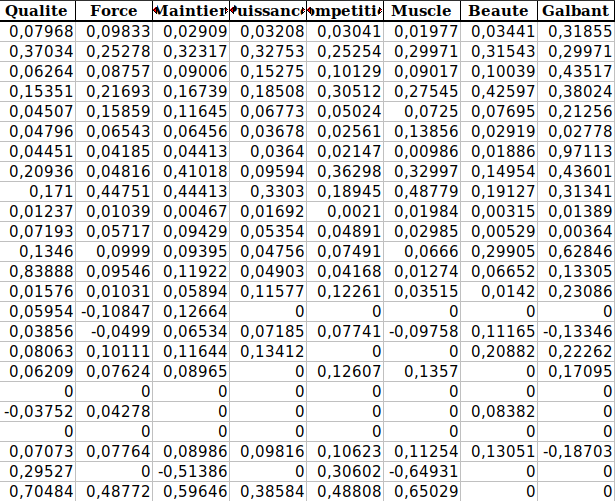
\includegraphics[scale=0.7]{donnée_nettoyé.png} 
\caption[]{Data \ processed }
\end{center}
\end{figure}

%%%% commenter l'image ( expliquer le sens des valeurs ) %%%%

Les mots les plus "importants"  et les moins "importants" pour chaque personne sont respectivement proche de soit 1 ou  de -1 et les moins "importants" sont proches de zero.

 The resulting data set contained 452
instances and 257 features.




\section{Clustering}  %%%%  Clustering method used %%%%


\subsection{Principal component analysis}
L'analyse en composantes principales est une méthode de la famille de l'analyse des données et plus généralement de la
statistique multivariée, qui consiste à transformer des variables liées entre elles (dites « corrélées » en statistique) en nouvelles variables décorrélées les unes des autres. Ces nouvelles variables sont nommées « composantes principales » ou axes principaux. Elle permet au statisticien de résumer l'information en réduisant le nombre de variables.

Dans notre projet, nous allons utiliser ACP pour réduire la dimension des données en quelques variables et garder les données les plus importants 



Quelles valeurs font-ils  rejeter ? Le code suivant permet d'y repondre 

\begin{lstlisting}
############## Partie PCA ########

res.pca <- PCA(data_base ,graph = TRUE)
print(res.pca)
summary(res.pca)

# Visualisation et interprétation

# Valeurs propres / Variances
library("factoextra")
eig.val <- get_eigenvalue(res.pca)
eig.val

fviz_eig(res.pca, addlabels = TRUE, ylim = c(0, 50))


# Resultas de la PCA 
var <- get_pca_var(res.pca)
var
# Contributions des variables aux PC

head(var$contrib,10)

# Contributions of variables to PC1  #  top = 35 - 40
fviz_contrib(res.pca, choice = "var", axes = 1, top = 35) 

# Contributions of variables to PC2  #  top = 35 - 40
fviz_contrib(res.pca, choice = "var", axes = 2, top = 35) 

# Contributions of variables to PC3  #  top = 35 - 40
fviz_contrib(res.pca, choice = "var", axes = 3, top = 35) 

# Contributions of variables to PC4  #  top = 35 - 40
fviz_contrib(res.pca, choice = "var", axes = 4, top = 35) 

# Contributions of variables to PC5  #  top = 35 - 40
fviz_contrib(res.pca, choice = "var", axes = 5, top = 35) 


## les variables garder 
donne = var$contrib
dim1  <- donne[,1]
dim2  <- donne[,2]
dim3  <- donne[,3]
dim4  <- donne[,4]
dim5  <- donne[,5]

print(dim1)
res <- dim1[dim1 > mean(dim1)]
print(names(res))
res1 <- names(res)


print(dim2)
res <- dim2[dim2 > mean(dim2)]
print(names(res))
res2 <- names(res)


print(dim3)
res <- dim3[dim3 > mean(dim3)]
print(names(res))
res3 <- names(res)


print(dim4)
res <- dim4[dim4 > mean(dim4)]
print(names(res))
res4 <- names(res)


print(dim5)
res <- dim5[dim5 > mean(dim5)]
print(names(res))
res4 <- names(res)

col_keep <- union(res1,res2)
col_keep <- union(col_keep,res3)
col_keep <- union(col_keep,res4)

print(col_keep)

\end{lstlisting}

\newpage

 


\begin{figure}[H]
\begin{center}
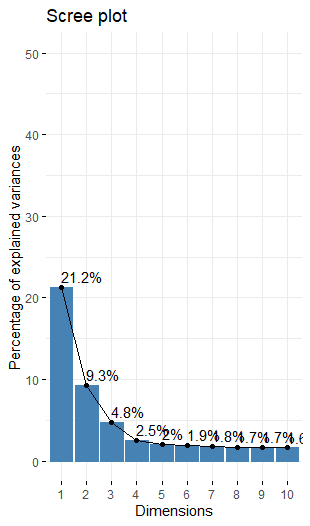
\includegraphics[scale=1.4]{ACP_1.png} 
\caption[]{\ }
\end{center}
\end{figure}

D'après le graphique ci-dessus, nous pourrions vouloir nous 
arrêter à la cinquième composante principale () car la variation est plus faible ).
Cependant 39.79760 \% des informations (variances) contenues 
dans les données sont retenues par les 5  premières composantes principales.



\begin{figure}[H]
\begin{center}
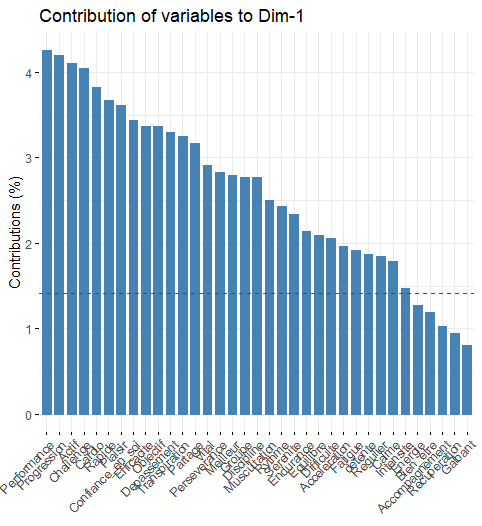
\includegraphics[scale=1.3]{ACP_2.png} 
\caption[]{\ }
\end{center}
\end{figure}



\begin{figure}[H]
\begin{center}
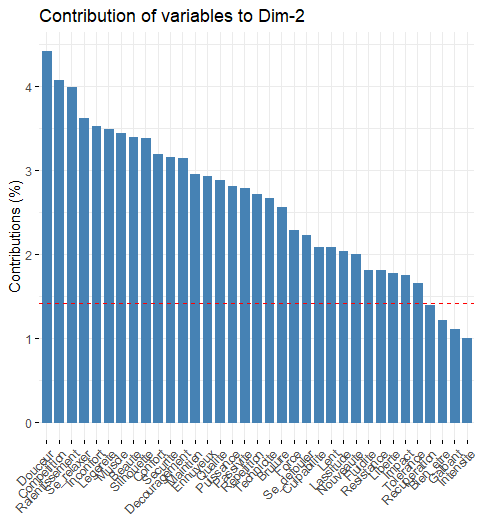
\includegraphics[scale=1.3]{ACP_3.png} 
\caption[]{\ }
\end{center}
\end{figure}


\begin{figure}[H]
\begin{center}
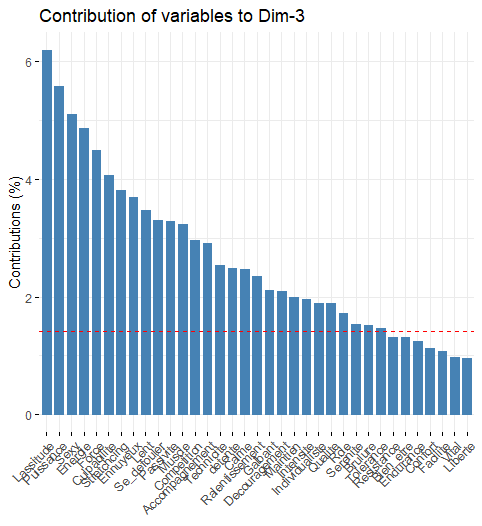
\includegraphics[scale=1.3]{ACP_4.png} 
\caption[]{\ }
\end{center}
\end{figure}


\begin{figure}[H]
\begin{center}
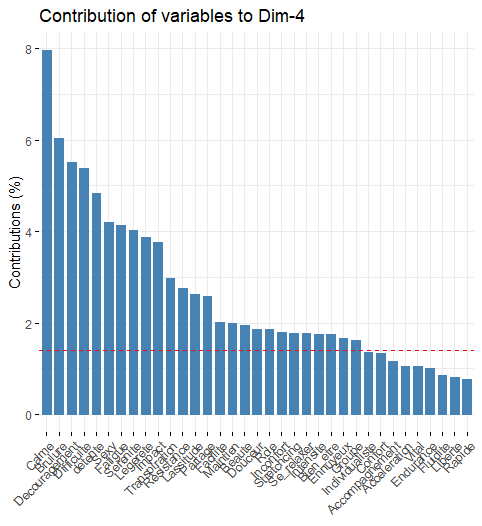
\includegraphics[scale=1.3]{ACP_5.png} 
\caption[]{\ }
\end{center}
\end{figure}


\begin{figure}[H]
\begin{center}
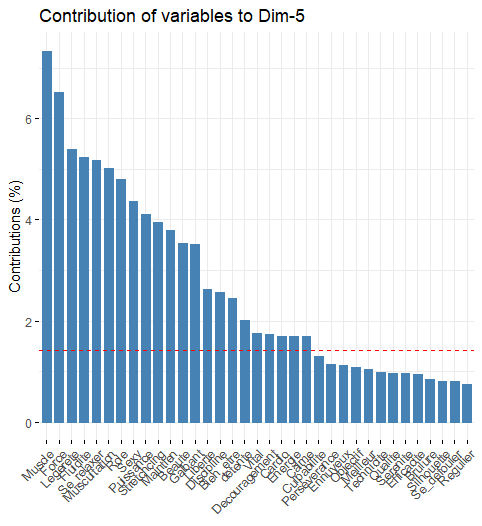
\includegraphics[scale=1.3]{ACP_6.png} 
\caption[]{\ }
\end{center}
\end{figure}


Maintenant que les variables les plus importantes ont ete conserve passons au algorithm de  clustering . Les variables délaisser par l'ACP sont les suivantes : "Recuperation" et  "Facilite"



\newpage   


\subsection{Hierarchical Clustering on Principal Components }  
L' approche HCPC ( Hierarchical Clustering on Principal Components ) permet de combiner les trois méthodes standards utilisées dans les analyses de données multivariées :

Méthodes en composantes principales (PCA, CA, MCA, FAMD, MFA),
Regroupement hiérarchique et
Clustering de partitionnement, en particulier la méthode des k-moyennes.





L'algorithme de la méthode HCPC a 4 principales étapes :

- Compute principal component methods: A cette étape, vous pouvez choisir le nombre de dimensions à retenir dans la sortie en spécifiant l'argument ncp .

Compute hierarchical clustering: Le regroupement hiérarchique est effectué en utilisant le critère de Ward sur les composantes principales sélectionnées. Le critère de Ward est utilisé dans le clustering hiérarchique car il est basé sur la variance multidimensionnelle comme l'analyse en composantes principales.

Choose the number of clusters based on the hierarchical tree: Un premier partitionnement est effectué en coupant l'arbre hiérarchique.

Perform K-means clustering : pour améliorer la partition initiale obtenue à partir du clustering hiérarchique. La solution finale de partitionnement, obtenue après consolidation avec k-means, peut être (légèrement) différente de celle obtenue avec le clustering hiérarchique.

Voici les lignes de codes utiliser dans le projet :

\begin{lstlisting}

res.pca <- PCA(data_base , ncp = 5 ,graph = TRUE)
res.hcpc <- HCPC(res.pca,nb.clust=3,consol=FALSE,graph=TRUE)

plot(res.hcpc,choice = "tree")
plot(res.hcpc,choice = "map", draw.tree = FALSE)
plot(res.hcpc,choice = "3D.map")
catdes(res.hcpc$data.clust,ncol(res.hcpc$data.clust))


# The original data with a column called clust 
# containing the partition
res.hcpc$data.clust

# Description of the clusters by the variables
s <- res.hcpc$desc.var
res.hcpc$desc.var


# Description of the clusters by the individuals
res.hcpc$desc.ind

\end{lstlisting}

\begin{figure}[H]
\begin{center}
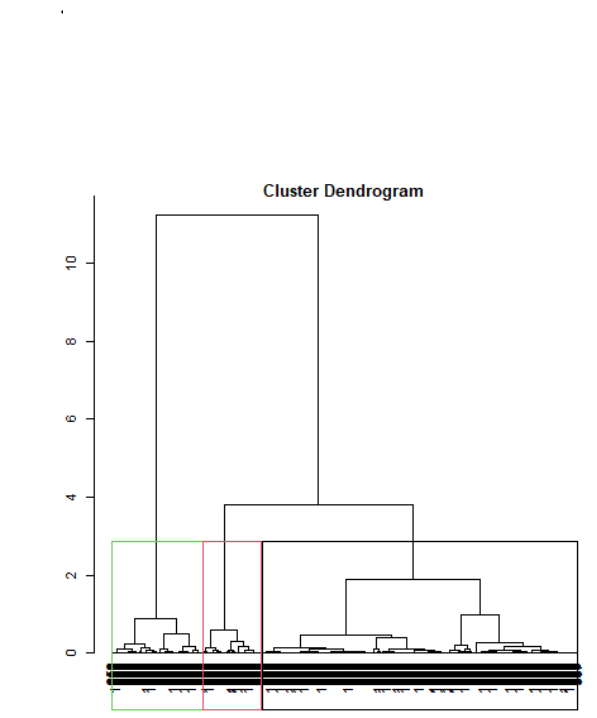
\includegraphics[scale=0.65]{classification_1.png} 
\caption[]{Hierarchical \ tree}
\end{center}
\end{figure}


\begin{figure}[H]
\begin{center}
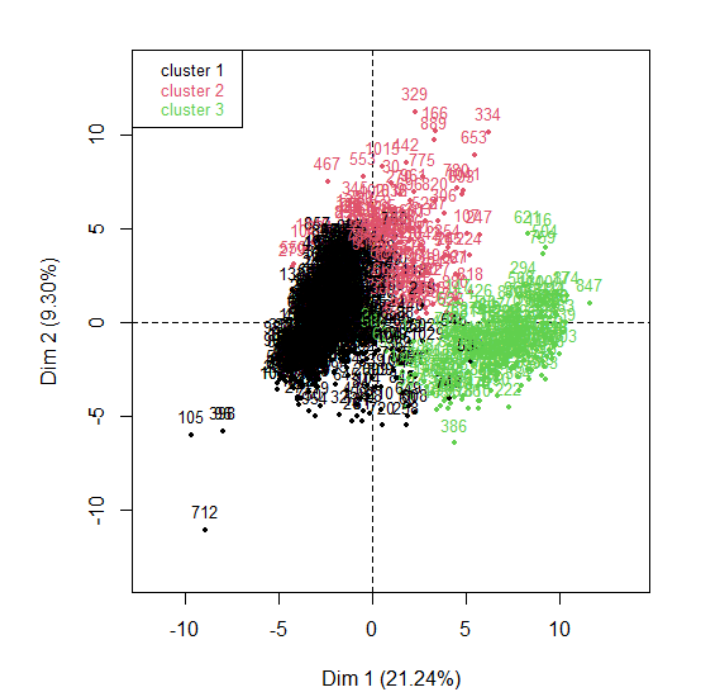
\includegraphics[scale=0.7]{classification_2.png} 
\caption[]{Ascending \ Hierarchical \ Classification \ of \ the \ individuals }
\end{center}
\end{figure}

\begin{figure}[H]
\begin{center}
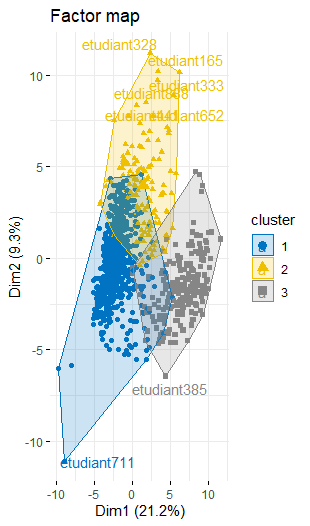
\includegraphics[scale=0.8]{hcpc.png} 
\caption[]{Ascending \ Hierarchical \ Classification \ of \ the \ individuals }
\end{center}
\end{figure}



The cluster 1 is made of individuals sharing :

- high values for the variables  Galbant, Culpabilite, Ennuyeux, 
Stretchcing, Securite, Decouragement, Ralentissement, Lassitude,
Inconfort et Passivite (variables are sorted from the strongest).

- low values for variables like Progression, Transpiration, Performance,
Actif, Challenge, Plaisir, Objectif, Perseverance, Confiance en soi and Cardio 
(variables are sorted from the weakest).


The cluster 2 is made of individuals sharing :


-	high values for variables like Se defouler, Puissance, Competition, Technicite, Qualite, Energie, Confort, Muscle, Force and Intensite (variables are sorted from the strongest).

-	low values for the variables Sexy, Meilleur, Calme and Vital (variables are sorted from the weakest).


The cluster 3 is made of individuals sharing :


-	high values for variables like Progression, Actif, Performance, Challenge, Cardio, Partage, Plaisir, Depassement, Rapide and Efficacite (variables are sorted from the strongest).

-	low values for variables like Confort, Securite, Galbant, Douceur, Ennuyeux, Force, Maintien, Qualite, Beaute and Inconfort (variables are sorted from the weakest).





\newpage


\section{Classification}  %%%%  Testing the strength of clusters %%%%

\subsection{Classification method} 
. expliquer la demarche 

Les données train ont été séparées  en 3 part : train , validation ,test.
Ligne de commande :

\begin{small}

\begin{lstlisting}
df = pd.read_csv("/home/congo/Bureau/2022-m1-staps/data_motives/clustering.csv") 

y = df.loc[:,'cluster3']

X = df
X.drop(df.columns[[0,1,2]], axis = 1, inplace = True)   

# separation des donnees en trois
train_ratio = 0.80
test_ratio = 0.10
validation_ratio = 0.10

size = validation_ratio/(train_ratio+test_ratio)

X_train,X_test,y_train,y_test=train_test_split(X,y,test_size=test_ratio)
X_train,X_val,y_train,y_val=train_test_split(X_train,y_train,test_size=size)

\end{lstlisting}
\end{small}


\setlength{\parindent}{0pt} Les donnees de validation serviront pour suprimer les valeurs a faible variance et  le seuil a ete fixe à 0.05 .

\setlength{\parindent}{0pt} Voici la commande utiliser pour la réaliser : 

\begin{lstlisting}
# elemination des colonnes a variances inferieur au seuil 0.1 ou 0.05
selector = VarianceThreshold(threshold=0.05)
selector.fit_transform(X_valid)
columns_selected = np.array(X_val.columns)[selector.get_support()] 
print(columns_selected)
\end{lstlisting}
En ce qui concerne les données de test 



\subsection{Results of Classification} 
. presentation des resultats


\section{Results and Conclusion}


\begin{thebibliography}{9}


\bibitem{texbook}
Donald E. Knuth (1986) \emph{The \TeX{} Book}, Addison-Wesley Professional.

\bibitem{lamport94}
Leslie Lamport (1994) \emph{\LaTeX: a document preparation system}, Addison
Wesley, Massachusetts, 2nd ed.


\end{thebibliography}

\end{document}